\documentclass[journal]{packages/vgtc}                % final (journal style)
%\documentclass[review,journal]{packages/vgtc}         % review (journal style)
%\documentclass[widereview]{packages/vgtc}             % wide-spaced review
%\documentclass[preprint,journal]{packates/vgtc}       % preprint (journal style)
%\documentclass[electronic,journal]{packages/vgtc}     % electronic version, journal

%% Uncomment one of the lines above depending on where your paper is
%% in the conference process. ``review'' and ``widereview'' are for review
%% submission, ``preprint'' is for pre-publication, and the final version
%% doesn't use a specific qualifier. Further, ``electronic'' includes
%% hyperreferences for more convenient online viewing.

%% Please use one of the ``review'' options in combination with the
%% assigned online id (see below) ONLY if your paper uses a double blind
%% review process. Some conferences, like IEEE Vis and InfoVis, have NOT
%% in the past.

%% Please note that the use of figures other than the optional teaser is not permitted on the first page
%% of the journal version.  Figures should begin on the second page and be
%% in CMYK or Grey scale format, otherwise, colour shifting may occur
%% during the printing process.  Papers submitted with figures other than the optional teaser on the
%% first page will be refused.

%% These three lines bring in essential packages: ``mathptmx'' for Type 1
%% typefaces, ``graphicx'' for inclusion of EPS figures. and ``times''
%% for proper handling of the times font family.

% TVCG Packages
\usepackage{mathptmx}
\usepackage{graphicx}
\usepackage{times}

\usepackage{multirow}
\usepackage{booktabs}
\usepackage{amsmath}
\usepackage{caption}
\usepackage{subcaption}
\usepackage[utf8]{inputenc}

% Import other packages
% Extra Packages
\usepackage{url}
\usepackage{epstopdf}
\usepackage{arydshln} % For \hdashline in tables
\usepackage{enumitem} % For [noitemsep] in lists

% Coloring author comments
\usepackage{color}
\usepackage[usenames,dvipsnames]{xcolor}
\definecolor{Purple}{rgb}{.75,0,.85}

\newif\ifnotes
\notestrue
\newcommand{\todo}[1]{\ifnotes {\textcolor{Purple}{\bf TODO: #1\ }} \fi}

% if we want to put in page breaks to assess length
\newif\iftestbreaks
\testbreakstrue
\newcommand{\testbreak}{\iftestbreaks\newpage\fi}

% Useful abbreviations
\usepackage{xspace}
\newcommand{\etal}{\emph{et al.}\@\xspace}
\newcommand{\ie}{\emph{i.e.}\xspace}
\newcommand{\eg}{\emph{e.g.}\xspace}
\newcommand{\etals}{\mbox{\emph{et~al.}'s }}

% TODO NSF CRI / Gleicher commands
\def\naive{na\"{\i}ve}
\def\naively{na\"{\i}vely}

% Droid Sans font
%\usepackage[defaultsans]{droidsans}
%\renewcommand*\familydefault{\sfdefault} %% Only if the base font of the document is to be typewriter style
%\usepackage[T1]{fontenc}
%\linespread{1.1}


\newcommand\map{
	
	\begin{figure}
		\centering
		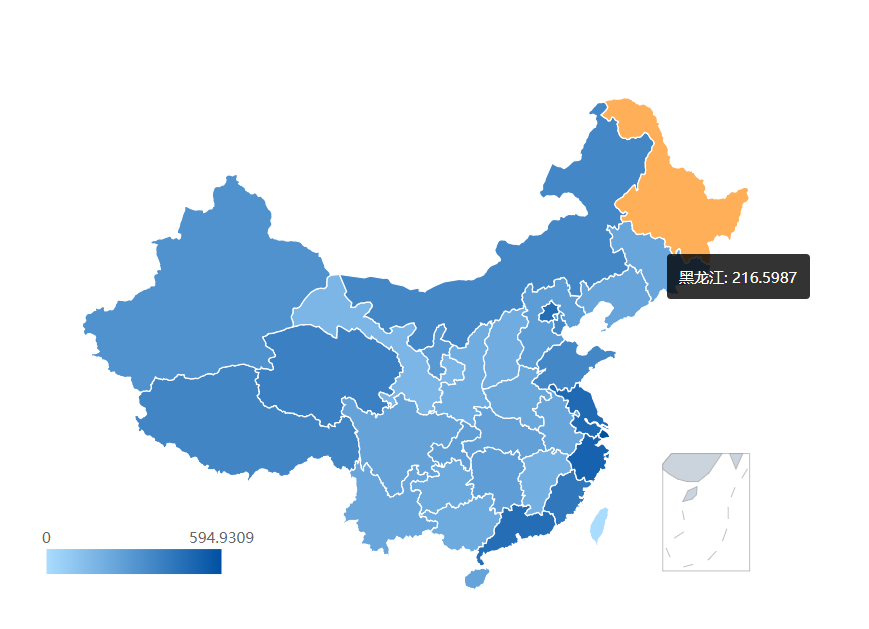
\includegraphics[width=\columnwidth]{img/map}
		\caption{
			In 2017, pre graduate number in China provinces. \S\ref{sec:results}
		}
		\label{fig:protein-validate}
	\end{figure}
	
}

\newcommand\timeline{
	
	\begin{figure}
		\centering
		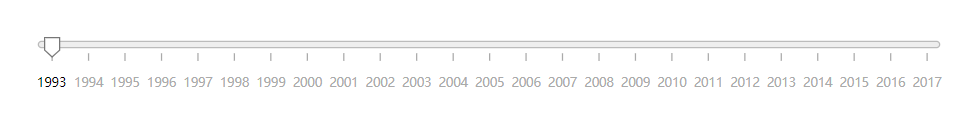
\includegraphics[width=\columnwidth]{img/timeline}
		\caption{
			Timeline from 1993 to 2017.
		}
		\label{fig:protein-validate}
	\end{figure}
	
}



% Import Tables
%%\input{tables.tex}

%% We encourage the use of mathptmx for consistent usage of times font
%% throughout the proceedings. However, if you encounter conflicts
%% with other math-related packages, you may want to disable it.

%% This turns references into clickable hyperlinks.
\usepackage[bookmarks,backref=true,linkcolor=black]{hyperref} %,colorlinks
\hypersetup{
  pdfauthor = {},
  pdftitle = {},
  pdfsubject = {},
  pdfkeywords = {},
  colorlinks=true,
  linkcolor= black,
  citecolor= black,
  pageanchor=true,
  urlcolor = blue,
  plainpages = false,
  linktocpage
}

%% If you are submitting a paper to a conference for review with a double
%% blind reviewing process, please replace the value ``0'' below with your
%% OnlineID. Otherwise, you may safely leave it at ``0''.
\onlineid{0}

%% declare the category of your paper, only shown in review mode
\vgtccategory{Research}

%% allow for this line if you want the electronic option to work properly
\vgtcinsertpkg

%% In preprint mode you may define your own headline.
%\preprinttext{To appear in an IEEE VGTC sponsored conference.}

%% Paper title.

\title{Education funding and undergraduates in different provinces in China}

%% This is how authors are specified in the journal style

%% indicate IEEE Member or Student Member in form indicated below
\author{Longsheng Xie \& Yuxiao Peng \& Zhaohui Li}



%% Abstract section.
\abstract{
Educational access remains uneven in China. Students born into affluent families generally have greater access to high-quality education than those from lower income backgrounds. So we decided to create a map of China and find the relationship between the data by comparing the education funds and the number of students in each province. And visulize the education funding \& undergraduate population in different area in a China map from 1993 to 2017. Then this paper will discuss how to create maps and data connections, and finally, show and discuss the final results and the goals that we want to accomplish in the future.
} % end of abstract

%% Keywords that describe your work. Will show as 'Index Terms' in journal
%% please capitalize first letter and insert punctuation after last keyword
\keywords{Map \& Data Visualization \& China \& Education \& Funding}

%% ACM Computing Classification System (CCS). 
%% See <http://www.acm.org/class/1998/> for details.
%% The ``\CCScat'' command takes four arguments.

\CCScatlist{ % not used in journal version
 \CCScat{K.6.1}{Management of Computing and Information Systems}%
{Project and People Management}{Life Cycle};
 \CCScat{K.7.m}{The Computing Profession}{Miscellaneous}{Ethics}
}

%% Uncomment below to include a teaser figure.
% Teaser should be jnds for -pcp versus +pcp (distinguishable; not distinguishable; target; not distinguishable; distinguishable)



%% Uncomment below to disable the manuscript note
%\renewcommand{\manuscriptnotetxt}{}

%% Copyright space is enabled by default as required by guidelines.
%% It is disabled by the 'review' option or via the following command:
% \nocopyrightspace

%%%%%%%%%%%%%%%%%%%%%%%%%%%%%%%%%%%%%%%%%%%%%%%%%%%%%%%%%%%%%%%%
%%%%%%%%%%%%%%%%%%%%%% START OF THE PAPER %%%%%%%%%%%%%%%%%%%%%%
%%%%%%%%%%%%%%%%%%%%%%%%%%%%%%%%%%%%%%%%%%%%%%%%%%%%%%%%%%%%%%%%%
\teaser{
	\centering
	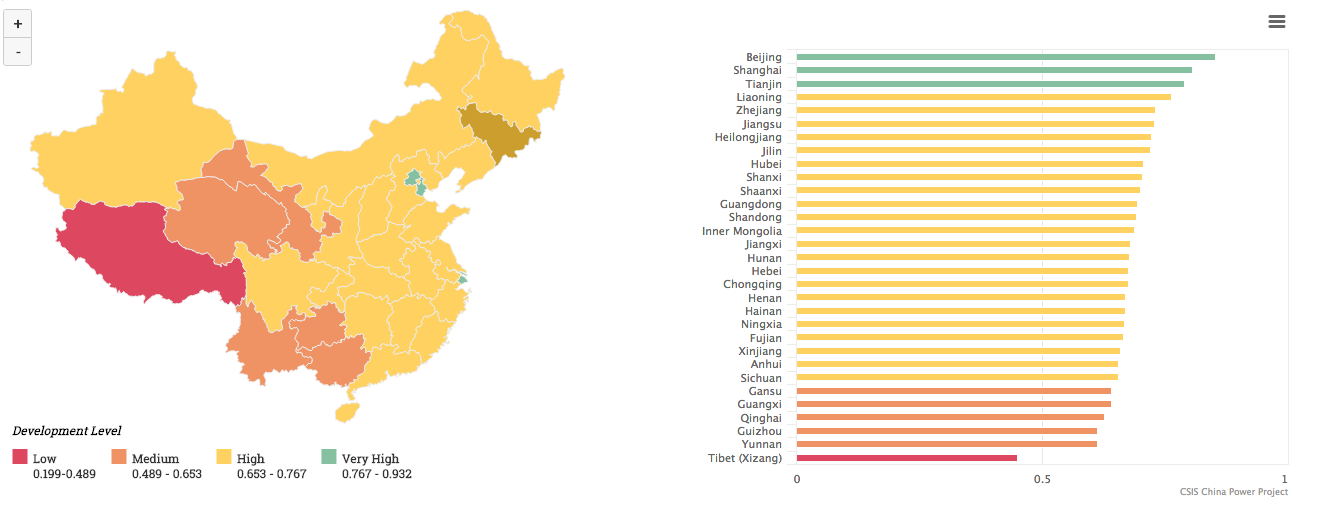
\includegraphics[width=\textwidth]{img/china}
	\caption{The relationship between provinces and education funding}
	\label{fig:teaser}
}

\begin{document}

%% The ``\maketitle'' command must be the first command after the
%% ``\begin{document}'' command. It prepares and prints the title block.

%% the only exception to this rule is the \firstsection command
\firstsection{Introduction}

\maketitle

%% \section{Introduction} %for journal use above \firstsection{..} instead

% Introduction section is automatically added

The objective of this paper is to analyze the educational funding and undergraduate population in each province in China at National Bureau of Statistics of China and found exponential increasing of the two attributes while the funding per undergraduate was fluctuating. It may reflect the focus changing from quantity to quality towards education in different areas. For example, a new policy from the government: In 1985, the government abolished tax-funded higher education, requiring university applicants to compete for scholarships based on academic ability. In the early 1980s, the government allowed the establishment of the first private institution of higher learning, increasing the number of undergraduates and people who hold doctoral degrees fivefold from 1995 to 2005..\cite{chen2000determinants}\\

\noindent In this project, we decided to create a map of China and find the relationship between the data by comparing the education funds and the number of students in each province. The purpose of this paper is to let people know about the changes and progress in China over the past 20 years. \cite{esteban2014lived}And this paper will discuss how to create maps and data connections, and finally, show and discuss the final results and the goals that we want to accomplish in the future.

\section{Background}
Innovation is a critical component of national power. It propels countries to develop new products or methods of production that drive economic progress and enable states to tackle transnational challenges, such as climate change and global health crises. The ability of a country to cultivate its capacity for innovation rests with its domestic education system. A well-educated workforce is instrumental to technological and scientific discovery, which can propel states to the apex of the increasingly innovation-based global economy.\\

\noindent Yet educational access remains uneven in China. Students born into affluent families generally have greater access to high-quality education than those from lower income backgrounds.\cite{rong2001inequality} Data from the National Bureau of Statistics suggest that urban residents in China enjoy a nearly threefold income advantage over their rural counterparts. The household registration system (hukou) has further widened this development gap by restricting the internal movement of persons.  Education-finance policies requiring local governments to bear partial responsibility for funding schools have compounded this issue, leaving less affluent areas without sufficient resources to pay skilled teachers, purchase necessary instruction materials, and maintain school faLiteracy is a baseline indicator of educational access. High levels of literacy serve as the foundation for improved access to information and directly enhance an individual’s ability to contribute to society.  As of 2011, China had all but eliminated illiteracy among young and middle-aged citizens – a landmark achievement for a country with the world’s largest population. Nevertheless, provincial variations reveal the incomplete nature of China’s ongoing development. Wealthy cities, such as Beijing and Shanghai, reported 2014 literacy rates (98.52 percent and 96.85 percent) comparable with those of developed countries.\cite{tsang1996financial} At the other extreme, Tibet’s literacy rate was a mere 60.07 percent in same year, pegging it closer to under-developed countries like Haiti and Zambia.

\section{Method}
We download the data from the National Bureau of Statistics of China (http://data.stats.gov.cn). It includes three csv: funds, undergraduate and per graduate. Each of them contains the data of each province in china from 1993 to 2017. funds.csv is the education funding for each province and undergraduate.csv contains the population in each province. Per graduate.csv is their divisor and it is the main data we focused on.\\

\noindent First, before we are doing the data visualization part, we think it is a good idea to see the relationship by the data, we want to see some interesting relation with the data, so we use the python to deal with the data. \cite{yu1977exploratory}We plot some line charts for each csv and compare of them so it can clearly show the change from the data.\cite{pedregosa2011scikit}\\

\noindent Then, in order to show the relationship between the educational funding and undergraduate population in each province in China. \cite{graves2013visualization}We think a contrast of color is a good way to compare of it on a real map rather than just show the bar chart by some tools like excel. \cite{bao2014visual}It is clearly to show the rate of change by the year and multiple views with other such graphs are better for analysis. So first we plot a map of China by d3 and link the raw per graduate data to each province, the color stand the data of each province and which color is darker for one province means the data is bigger, we also plot a scale in the bottom so you can see which color stand for which data.\cite{harper2014deconstructing} \\

\noindent Besides, we also want to plot a time slider in the website\cite{wang2008importance}, when you choose other year in the slider, the color will change to the data of that year\cite{healey1996choosing}, so the color and scale will change. \cite{zastrow2015data}So you can see whether the data is increase or decrease for each province.\\

\noindent Finally, we analyses the data for each province to see any interesting thing, Specifically, the change in number of funds and the amount of population of undergraduate is compared over the years to see the relationships of them,\cite{tsang1996financia} and which province put the most funding to education and get more people undergraduate.

\timeline

\section{Results}
\label{sec:results}

\map

The funding and undergraduate students are increasing sharply from 1993 to 2017 while the funding per undergraduate goes a 'S' curve. That's very interesting things to show the changing of education department of China's focus on the quality or the quantity of the students. While that's the overall changing of the education funding. The specific situations in different provinces are different. So we want to visualize the funding per undergraduate changing in different provinces to find out some interesting things.

\section{Discussion}
By comparing and analyzing the actual situation, we know that the environmental conditions in each province have been very different from ancient times to the present, so the current investment in education cannot explain the importance that the province attaches to education. Geographically, the geographical location of the province (whether coastal or not) is an important factor affecting whether students choose to go to the province, and the province with convenient transportation has a good economic foundation, so there will be a higher investment in education. Historically, if the province has a high historical status in the development of China before, there will be many long-established and relatively good schools, so the investment in education will also occupy a large proportion. Moreover, China's population distribution is extremely uneven. Although some provinces have a lot of investment in education, their investment in each student is very limited due to their large population base. This is also a major reason for restricting the development of education in some provinces.\\

\noindent If there is plenty of time, we want to combine the visualization of the map with specific data and timelines so that we can see how the province has invested in education for a long time. In the future, we will try our best to combine this map with the 3D histogram to present the top view of the map. \cite{du20043}The investment in education and the number of students will be displayed through a 3d histogram, which shows the difference between provinces more clearly and intuitively\cite{satyanarayan2014declarative}.

\section{Conclusion}
\label{sec:conclusion}

The project aimed at the education budget and undergraduate population of the National Bureau of Statistics in China, and found that these two attributes increased exponentially, while the upstream of each college student was fluctuating. It may reflect a shift in the number of education from different to quality. \cite{dougherty1995supervised}From 1993 to 2017, although there are only 24 years of data, it is enough to get China's rapid emphasis on education in China's rapid development. In economically developed provinces, education investment also accounts for a larger proportion, so it is concluded that education and the economy are positively related.\\

\noindent In the future, collecting more comprehensive economic and educational data, we can get a more accurate analysis.\cite{dibiase1992animation} For example, the province’s main source of income will not affect the proportion of education investment in the province and will affect the province’s major educational resources. Next, we will also upgrade from a 2d map to a 3d map, making the entire visualization clearer and more intuitive. 


%% if specified like this the section will be committed in review mode
\acknowledgments{
The Authors would like to acknowledge Lane Harrison for his insight in improving ideas throughout the project.
}
\bibliographystyle{abbrv}
\bibliography{paper.bib}


\end{document}
